\section{776 --- Split BST}
Given a Binary Search Tree (BST) with root node \fcj{root}, and a target value $V$, split the tree into two subtrees where one subtree has nodes that are all smaller or equal to the target value, while the other subtree has all nodes that are greater than the target value.  It's not necessarily the case that the tree contains a node with value $V$.

Additionally, most of the structure of the original tree should remain.  Formally, for any child \textbf{C} with parent \textbf{P} in the original tree, if they are both in the same subtree after the split, then node \textbf{C} should still have the parent \textbf{P}.

You should output the root \fcj{TreeNode} of both subtrees after splitting, in any order.

\paragraph{Example 1:}
\begin{flushleft}


\textbf{Input}: \fcj{root = [4,2,6,1,3,5,7]}, \fcj{V = 2}

\textbf{Output}: \fcj{[ [2,1], [4,3,6,null,null,5,7] ]}

\textbf{Explanation}:

Note that \fcj{root}, \fcj{output[0]}, and \fcj{output[1]} are TreeNode objects, not arrays.

The given tree \fcj{[4,2,6,1,3,5,7]} is represented by the following diagram:

\begin{figure}[H]
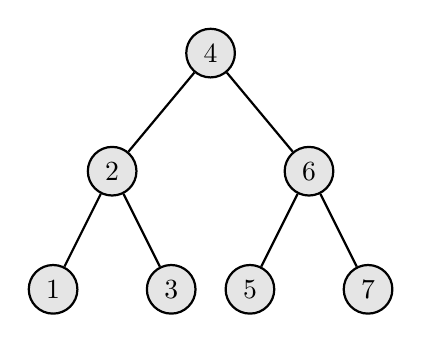
\begin{tikzpicture}
[every node/.style={draw, circle, fill=gray!20!, minimum size=5mm},
level 1/.style={sibling distance=25mm},
level 2/.style={sibling distance=15mm},
thick]
\node{4}
child{node{2} child{node{1}} child{node{3}}}
child{node{6} child{node{5}} child{node{7}}};
\end{tikzpicture}
\end{figure}

while the diagrams for the outputs are:

\begin{figure}[H]
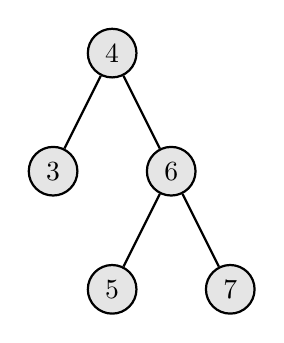
\begin{tikzpicture}
[every node/.style={draw, circle, fill=gray!20!, minimum size=5mm},
%level 1/.style={sibling distance=25mm},
%level 2/.style={sibling distance=15mm},
thick]
\node{4}
child{node{3} child[missing]}
child{node{6} child{node{5}} child{node{7}}};
\end{tikzpicture}
\end{figure}

and

\begin{figure}[H]
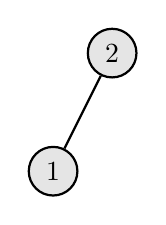
\begin{tikzpicture}
[every node/.style={draw, circle, fill=gray!20!, minimum size=5mm},
%level 1/.style={sibling distance=25mm},
%level 2/.style={sibling distance=15mm},
thick]
\node{2}
child{node{1}}
child[missing];
\end{tikzpicture}
\end{figure}

\end{flushleft}

\paragraph{Note:}

\begin{itemize}
\item The size of the BST will not exceed 50.
\item The BST is always valid and each node's value is different.
\end{itemize}

\subsection{Recursion}
For each \fcj{node} in the BST, it either belongs to the first half or the second half. Assume it belongs to the first half.

Based on the property of BST, the entire subtree at \fcj{node.left} must be in the first half. However, the subtree at \fcj{node.right} may have nodes in either halves, so it needs to be split.

We get the split result $t$ by recursively calling the function \fcj{split(node.right)}. Since \fcj{t[0]} and \fcj{t[1]} are also BST, $t[0]$ must be in the first half, and it must be to the right of \fcj{node} for the first half to be a BST. Then $t[1]$ is the second half.

\setcounter{lstlisting}{0}
\begin{lstlisting}[style=customc, caption={Recursion}]
vector<TreeNode*> splitBST( TreeNode* root, int V )
{
    if( !root )
    {
        return {nullptr, nullptr};
    }
    if( root->val <= V )
    {
        //we need to split right subtree
        auto two_trees = splitBST( root->right, V );
        //set root->right as the left part
        root->right = two_trees[0];
        //root is put in the left part
        two_trees[0] = root;
        return two_trees;
    }
    //root->val > V
    //we need to split left subtree
    auto two_trees = splitBST( root->left, V );
    //set root->left as the right part
    root->left = two_trees[1];
    //root is put in the right part
    two_trees[1] = root;
    return two_trees;
}
\end{lstlisting}